% Sample Dissertation, Thesis, or Document %
%            for use with the              %
%  University of Arizona Thesis Class,     %
%               uathesis.cls               %
%------------------------------------------%

% We'll use the uathesis document class (duh).  The uncommented line
% below will produce a Dissertation, the others would produce a Thesis
% or a Document.  There are other options available to you like turning
% on the copyright statement and replacing the year on the title page
% with a "generated on" stamp (handy for early drafts).  To find out
% what the available options are, take a look into the uathesis.cls
% file and look for the \DeclareOption commands near the top of that
% file.
% There are five copyright options.  Copyright, no copyright, and three
% different Creative Commons licences.  Use the one you want (If you go
% Creative Commons, I (DM) think the CC-BY-ND makes the most sense)  See
% uathesis.cls for the reason why the non-commercial licenses are not
% included.
\documentclass[dissertation]{uathesis}
%\documentclass[dissertation,copyright]{uathesis}
%\documentclass[dissertation,CC-BY]{uathesis}
%\documentclass[dissertation,CC-BY-SA]{uathesis}
%\documentclass[dissertation,CC-BY-ND]{uathesis}
%\documentclass[thesis]{uathesis}
%\documentclass[document]{uathesis}

% Package Usage
% These are the packages that we need
\usepackage{graphicx}
\usepackage{natbib}			% natbib is available on most systems, and is
					% terribly handy.
					% If you want to use a different Bibliography package, 
					% you should be able to, just change this
					% and the \bibliographystyle command below.  Be warned
					% that you may need to do a little hacking to get
					% the REFERENCES item to show up in your TOC.

% Compatibility with the AASTEX package 
% of the American Astronomical Society.
% I COMMENTED OUT LINE 150 OF DELUXETABLE.STY
\usepackage{deluxetable}		% Allows use of AASTEX deluxe tables
\usepackage{aastex_hack}		% Allows other AASTEX functionality.


% These are other packages that you might find useful.
% For controlling the fonts, see
% http://www.math.uiuc.edu/~hartke/computer/latex/survey/survey.html
% The following is a nice font set:
%\usepackage{mathtime}			% Times for letters; Belleek math.
%
\usepackage{amsmath}			% AMS Math (advanced math typesetting)
\usepackage{amssymb} 
\usepackage{lscape}			% Used for making fitting large tables in by putting them landscape
\usepackage[tableposition=t]{caption} % NICK ADDED THIS (makes table captions normal size when font set smaller)

%%% Evan added the following
\usepackage{mathtools}
\usepackage{bm}
\usepackage{enumitem}
\usepackage{units} % includes nicefrac

%%% The following allows dagger footnote on chapter titles
%%% with no number. Useful for designating previously 
%%% published work.
\newcounter{daggerfootnote}
\newcommand*{\daggerfootnote}[1]{%
    \setcounter{daggerfootnote}{\value{footnote}}%
    \renewcommand*{\thefootnote}{\fnsymbol{footnote}}%
    \footnote[2]{#1}%
    \setcounter{footnote}{\value{daggerfootnote}}%
    \renewcommand*{\thefootnote}{\arabic{footnote}}%
    }

\newcommand{\Msun}{\mathrm{M}_{\odot}}
%\usepackage{refs}			
%
% If you are using hyper-ref (recommended), this command must go after all 
% other package inclusions (from the hyperref package documentation).
% The purpose of hyperref is to make the PDF created extensively
% cross-referenced.
\usepackage[hidelinks]{hyperref}


% Set up some values.
\completetitle{Magnetic Reconnection in Low-Luminosity Accretion Flows: from Microphysical Simulations to Large-Scale Models}
\fullname{David Ramsey Ball}			% Grad college wants your full name here.
\degreename{Doctor of Philosophy}	% Title of your degree.
\degreemajor{Astronomy and Astrophysics} % Degree major
\begin{document}


% Set up the title page
\maketitlepage
{University of Arizona Department of Astronomy}	% Title of your department.
{2020}							

% Insert the approval form.  Note that for electronic submission
% of your Ph. D. dissertation, you must bring *two* copies of the
% approval page to your final defense.  These must be signed by
% the committee.  Make two photocopies: one for Pam and the other
% for your records.  Then, bring the two signed originals to the
% graduate college when you submit the final version of the
% dissertation to the University of Arizona.
\approval
{}		% Defense Date	
{}	% Dissertation Director
{}	% 1st committee member
{}		% 2nd committee member
{}		% 3rd committee member
{}		% 4th committee member
{}		% 5th committee member
{}		% 6th committee member

% Include the ``Statement by Author'' for Dissertations
\statementbyauthor
% If this is a Thesis, use the following form, with your thesis director's
% name and title in the square brackets like so (you should also omit the 
% approval form insertion above):
%\statementbyauthor[Jane M. Doe\\Professor of Chemistry]

% Include the ``Acknowledgements''
\incacknowledgements{acknowledgements}

% Include the ``Dedication''
\incdedication{dedication}

% Create a ``Table of Contents''
\tableofcontents

% Create a ``List of Figures''
%\listoffigures

% Create a ``List of Tables''
%\listoftables

% Include the ``Abstract''
\incabstract{abstract}

% Include the various chapters
\chapter[Introduction]
{Introduction}
%\begin{figure}
%\centering
%\includegraphics[angle=0,width=\columnwidth]{fig1.pdf}
%\caption[]{}
%\label{fig1}
%\end{figure}
\section{Black Holes and Accretion}

Black holes have drawn substantial attention from both scientists and the public since Karl Schwarzchild first formulated them as a solution to Einstein's field equations (\citealt{schwarzschild1916}).  Since then, scientists have generated a massive body of work focused on understanding these captivating objects and the material that collects around them.  In this dissertation, we will focus on understanding the physics of hot ionized gas (or, plasma) that swirls around black holes and heats up to extremely high temperatures, lighting up the direct surroundings of black holes at nearly all wavelengths, from the radio to X-ray.  

Black holes range in size, from just over the mass of the Sun ($3.8 M_{\rm{sun}}$, \citealt{smallbh}), to over a billion times the mass of the Sun ($6.5\times10^9 M_{\rm{sun}}$, e.g., \citealt{eht6}).  We will focus on so-called ``supermassive black holes" (defined for our purposes as $M>10^6 M_{\rm{sun}}$).  Supermassive black holes can have profound impacts on their environments and are responsible for a variety of critical phenomena in terms of galaxy evolution.  For instance, the supermassive black hole at the center of M87 is thought to be responsible for generating powerful jets that we see emerging from a very compact source in this galaxy (reference).  More recently, this black hole was imaged by the Event Horizon Telescope collaboration (EHT) and showed the telltale sign of the ``black hole shadow'' imprinted on the surrounding material's emission.  By providing the first horizon-scale imaging of black holes, the EHT provides a new testbed not only for General Relativity, but also for our understanding of plasma physics in a regime that terrestrial experiments cannot probe.

The closest supermassive black hole to the Earth is Sagittarius A* (henceforth Sgr~A*), which resides at the center of our own Milky Way galaxy.  Numerous observing campaigns have been dedicated to characterizing the emission from this source, both in terms of its spectrum, as well as its variability (references).  These detailed observations, when combined with the appropriate physical models, are extremely powerful in furthering our understanding of the physics of these systems.  Sgr~A* is quite dim, and hence, is classified as a ``low-luminosity accretion flow'', and is thought to have a very low accretion rate $\sim 3 \times 10^{-5} \; \rm{M_{sun}} \; \rm{yr}^{-1}$ (e.g. \citealt{quataert1999b}).  We will elaborate further on the physics of low-luminosity accretion flows in section \ref{sec_lowlum}.

Observations of Sgr~A* reveal significant multiwavelength variability (see \citealt{eckart2004, marrone2008, neilsen2013, witzel2013, ponti2015, li2015, wang2016}) from the mm and IR to the X-rays.  At high energies, in particular, \citet{neilsen2013} analyzed 3 million seconds of Chandra data dedicated to characterizing both short and long-term X-ray variability of Sgr~A*.  They found that the length of flares varies from a few hundred seconds to 8 ks, with luminosities from $\sim 10^{34} \; \rm{erg} \; \rm{s}^{-1}$ to $2 \times 10^{35} \; \rm{erg} \;  \rm{s}^{-1}$.  More recently, \citet{haggard2019} quantified the behavior of some of the brightest X-ray flares, and showed that some of them have distinct double-peaked structures to the lightcurve.  \citet{eckart2004} carried out simultaneous observations in both the X-ray and near IR, and found that X-ray flares always have a coincident IR flare.  In contrast, there are numerous IR flares without X-ray counterparts.  These flares can offer unique insight into the particle energetics of the accretion flow; highly energetic stochastic flares point towards mechanisms such as shocks and magnetic reconnection, which are capable of quickly producing large numbers of high energy non-thermal particles which significantly alter the observational signatures of the accretion flow.

\section{Low-Luminosity Accretion Flows}
Many supermassive black holes, including Sgr~A*, have small accretion rates, and as a result, have very low luminosities.  In these systems, the radiative efficiency is low due to the low density of the plasma in the flow, and hence are often coined ``radiatively inefficient accretion flows'' (henceforth, RIAFs).  In contrast with relatively cold and radiatively efficient thin disk models, radiatively inefficient accretion flows remain very hot precisely because the energy carried away by radiation is negligible compared to the viscously dissipated energy in the system.  The high temperatures and low densities in these disks cause them to be geometrically thick and optically thin.  As such, their spectra are dominated by various emission processes such as synchrotron and bremsstrahlung that occur at different locations throughout the disk, resulting in spectra that deviate substantially from a simple blackbody.

The low plasma density in RIAFs has a number of interesting implications.  The timescale for electron-ion Coulomb collisions to exchange energy is longer than the heating timescale, which means that the electrons and ions likely have different temperatures.  Electrons are expected to be substantially colder than ions for a number of reasons: first, heating mechanisms such as the dissipation of turbulent (or magnetic) energy and shocks tend to favor the more massive species (\citealt{howes2010}, \citealt{rowan2017}) across a broad range of plasma parameters (with the exception of when the plasma-$\beta$, the ratio of gas to magnetic pressure, is very low), second, electrons radiate away their energy at a much faster rate than ions.  In addition to ions and electrons being thermally decoupled, electron-electron and ion-ion Coulomb collision timescales are also  longer than dynamical timescales, meaning the distribution function of each species may be highly nonthermal (i.e., deviating substantially from a Maxwellian).

The role of non-thermal electron energy distributions have been addressed in the context of stationary hydrodynamic models by \citet{mahadevan1998}, \citet{ozel2000}, and \citet{yuan2003}, who showed that even a relatively small number of power-law electrons can significantly impact the spectra predicted from a model, generating X-ray power-law tails as well as boosting the low frequency radio flux.  These studies used analytical steady-state solutions to calculate spectra, which do not capture short timescale GRMHD effects that play a large role in determining the variability properties of the system.  In section \ref{phenom_model}, we will elaborate further on the work that has been done to address nonthermal electrons in low-luminosity accretion flows, and describe a phenomenological model we developed to explain the X-ray flares from Sgr~A* in the framework of magnetohydrodynamic simulations and radiative transfer calculations.

\label{sec_lowlum}
\section{Magnetohydrodynamics}
While substantial work has been done to analytically understand the steady-state global solutions to RIAFs (see \citealt{yuan2014} for a recent review), these calculations make a number of simplifying assumptions.  In particular, in order to make the calculations tractable, most studies assume steady and axisymmetric accretion flows and also prescribe an artificial kinematic viscosity to enable accretion.  While these solutions are enlightening and highlight some of the basic underlying physics of accretion disks, they are not suited for studying the nonlinear physics of accretion, the turbulence that arises, and the associated variability in emission.  In order to understand these processes, we must turn to numerical simulations.

The most commonly used type of simulation to study accretion flows around black holes are ``general relativistic magnetohydrodynamic'' (henceforth GRMHD) simulations.  In short, these are simulations that capture the dynamics and energetics of an ionized gas in the static but curved spacetime around a black hole.  The framework of MHD makes a number of simplifying assumptions.  First, it assumes that the plasma satisfies the fluid approximation: that the collisional mean-free-path is much less than the scale of interest.  Most MHD simulations also utilize the ``ideal MHD'' approximation: that the plasma is infinitely conductive.  In other words, because electrons have such a small mass, they respond extremely rapidly to the presence of electric fields and will immediately short out any electric field in the system, ensuring that the fluid remains electrically neutral.  One consequence of the ideal MHD approximation is that it effectively ``freezes'' the magnetic field into the fluid, so that the evolution of the magnetic field is simply described as being advected around with the fluid.  In reality, the ideal MHD approximation drops a number of other higher-order terms to simplify the evolution of the magnetic field, we will now briefly cover how the evolution of the magnetic field evolves in the framework of ideal MHD and the assumptions used to get there.  For clarity, all of the following equations in this section are in the nonrelativistic limit, where the equations lend themselves far more readily toward building physical intuition.  We note, however, that the general principles we discuss also apply to the relativistic analogs.

We will begin by considering the generalized Ohm's law:

\begin{equation}
	\bold{E}+\bold{u}\times \bold{B} = 
	\eta \bold{J} + \frac{1}{e n}\left(\bold{J} \times \bold{B} - \nabla \cdot \overleftrightarrow{\bold{P}}_{e} + \frac{m_e}{e}\left[\frac{\partial \bold{J}}{\partial t}+\nabla \cdot (\bold{Ju} + \bold{uJ})\right]\right).
	\label{ohm}
\end{equation}

Here $\bold{E}$, $\bold{B}$, $\bold{u}$, and $\bold{J}$ represent the electric field, magnetic field, fluid velocity (the mass-weighted average velocity, including both species), and current, while $\overleftrightarrow{P_e}$ represents the electron pressure tensor.  In this dissertation, bolded quantities represent vectors while double arrows above a bold quantity represent rank-2 tensors.  The remaining quantities: $\eta$, $e$, $n$, and $m_e$ are simply the fluid's resistivity, the charge of a proton, the number density of the fluid, and electron mass.  In this equation, the first term on the right hand side is simply Ohmic dissipation. The first term in parenthesis is the so-called ``Hall'' term and the following two terms include effects from the divergence of the electron pressure tensor and electron inertial effects, all of which contribute to the electric field.  For most purposes, the terms within the parenthesis are neglected due to the small factor of $1/en$, which is typically negligible compared to the other terms in the equation in astrophysical contexts.  The ideal approximation sets the entire right hand side to 0 (by the argument that $1/en$ is very small, and that the electrical resistivity, $\eta$, is nearly 0, corresponding to an infinite conductivity $\sigma=1/\eta$).  This results in the much simpler expression for the electric field of

\begin{equation}
	\bold{E}_{\rm{ideal}}=-\bold{u}\times \bold{B}.
	\label{ideal_E}
\end{equation} 

This electric field is often referred to as the ``ideal'' or ``motional'' electric field, and can be understood simply as the electric field induced by moving magnetic fields.  In order to assess the evolution of the magnetic field, we plug the electric field found in \ref{ideal_E} into Faraday's law:

\begin{equation}
	\frac{1}{c}\frac{\partial \bold{B}}{\partial t} = - \nabla \times \bold{E_{\rm{ideal}}}=\nabla \times (\bold{u}\times\bold{B})
	\label{faraday}
\end{equation}

This leads to a phenomenon known as ``flux freezing'': it is relatively straightforward to show that Equation \ref{faraday} implies that the magnetic flux through a fluid element is conserved as the fluid moves.  Another related, although not identical implication is the so-called ``Lundquist Theorem'' that shows that Equation \ref{faraday} more generally describes how a any vector field (in this case, $\bold{B}$) is advected by a velocity field.  This means that the magnetic field can be stretched and compressed by fluid motions, but cannot reconnect or dissipate.

The underlying assumptions that lead to the equations of ideal MHD make the system of equations much more tractable to implement numerically.  Furthermore, the assumptions are quite sound for a large number of astrophysical systems and scales.  MHD (and GRMHD, when necessary) has proven to be a powerful tool over the last few decades and has explained a wide variety of astrophysical phenomena, from accretion on to black holes, to the behavior of plasma in the outskirts of galaxy clusters, to the solar wind and corona.

\subsection{Shortcomings of the MHD approximations}
While the fundamental assumptions of ideal MHD may be valid on the largest scales in the system, in principle, small regions may arise that violate the underlying assumptions.  For instance, if we consider the generalized Ohm's law (Equation \ref{ohm}) in the limit where the Hall, electron pressure tensor, and electron inertia terms are negligible, we get the ``resistive Ohm's law'',

\begin{equation}
\bold{E} + \bold{u} \times \bold{B} = \eta \bold{J}.
\end{equation}

In order to assess the importance of a finite resistivity on the evolution of the magnetic field, we once again plug the electric field into Faraday's law:


\begin{equation}
	\frac{1}{c}\frac{\partial \bold{B}}{\partial t} =\nabla \times (\bold{u}\times\bold{B}) -\nabla \times \eta \bold{J}
	\label{faraday_resistive}
\end{equation}
	
In the limit of nonrelativistic MHD, the current is simply the curl of the magnetic field, i.e.,

\begin{equation}
	\bold{J} = \frac{c}{4\pi}\nabla \times \bold{B}.
\end{equation}
As such, we can write the evolution of the magnetic field in terms of itself and the fluid velocity as 

\begin{equation}
	\frac{1}{c}\frac{\partial \bold{B}}{\partial t} =\nabla \times (\bold{u}\times\bold{B}) -\nabla^2 \eta \bold{B}.
\end{equation}
In most cases, we assume that the resistivity is roughly constant in space so that it simply acts as a diffusion coefficient via

\begin{equation}
		\frac{1}{c}\frac{\partial \bold{B}}{\partial t} =\nabla \times (\bold{u}\times\bold{B}) -\eta \nabla^2 \bold{B}.
\end{equation}

We see that the effect of a finite resistivity serves to dissipate the magnetic field.  In the ideal MHD assumption, we dropped the resistive term, arguing that $\eta$ is small.  Here, however, we see that even in the limit where $\eta$ is small, if regions arise where $\nabla^2 \bold{B}$ is large, then the $\eta \nabla^2 \bold{B}$ term may end up being dynamically and energetically important to this system.  One such type of configuration that may arise is a so-called ``current sheet'', where the magnetic field reverses its direction over a short length scale.  This configuration is unstable and prone to undergo magnetic reconnection, which we will describe in more detail in the following section and will be a focus of this dissertation.

\section{Magnetic Reconnection}
Magnetic reconnection is a fundamental plasma process in which opposing field lines in a plasma that are separated by a short distance rearrange their topology, connecting with one another.  In doing so, they release magnetic energy into the ambient plasma in the form of bulk motion, heat, and in some cases, particle acceleration.  Reconnection was first formulated in the context of resistive MHD by Eugene Parker and Peter Sweet in 1956 in an attempt to explain the dynamics of solar flares.  We will now briefly review a dimensional argument that follows their original formulations from \citet{parker1957} and \cite{sweet1958} and is widely known as the ``Sweet-Parker'' model of reconnection.  Because this is not a rigorous derivation, but rather a scaling argument, we will not concern ourselves much with factors of order unity, but instead focus on the underlying physics and trends that this model uncovers.

Consider a current sheet in which the x-component of the magnetic field, $B_x$, reverses direction over a distance of $\delta$ in the y-direction, and extends along a distance $L$ in the x-direction.  On either side of the layer, the strength of the magnetic field is $B$.  This geometry will have an associated current in the z-direction with a magnitude of 

\begin{equation}
	J_{\rm{z}} = \frac{c}{4 \pi}\frac{B}{\delta}.
\end{equation}    

Outside of the current sheet, the magnetic field strength is constant, and hence there is no current.  As such, the only electric field in this region is from magnetized plasma flowing towards the layer (in the y-direction), which will have a magnitude of $E_{\rm{outside}} \approx u_{\rm{in}}B$, where $u_{\rm{in}}$ is the inflow speed (the bulk velocity of plasma flowing towards the current layer in the y-direction).  Within the layer, the magnetic field goes to 0, so there is no ideal electric field.  There is, however, a current and finite resistivity.  As such, there will be a resistive electric field with magnitude 

\begin{equation}
E_{\rm{inside}} \approx \frac{c}{4\pi}\frac{\eta B}{\delta}.
\end{equation}

By matching $E_{\rm{inside}}$ to $E_{\rm{outside}}$, we can derive an expression for the inflow speed as a function of the other parameters in the setup,

\begin{equation}
	u_{\rm{in}} = \frac{c}{4 \pi} \frac{\eta B^2}{\delta}.
\end{equation}

In the geometry in which plasma is flowing towards the current layer in the outer region (in the y-direction), and plasma within the current sheet flows out along the x-direction, the equation of energy conservation of energy can be written as

\begin{equation}
	\frac{B^2}{4 \pi} = \frac{1}{2}\rho u_{\rm{out}}^2.
\end{equation}

From here, we see that the outflow speed is simply the Alfv\'en speed: 

\begin{equation}
	u_{\rm{out}}=\frac{B}{\sqrt{4\pi \rho}}
\end{equation}

With a bit algebra, it is straightforward to show that the inflow speed can be written simply as $\eta/\delta$, resulting in a reconnection rate that is far too slow to account for observed astrophysical phenomena.  While the Sweet-Parker model of reconnection is quite simplified and doesn't account for some important and relevant physics, it highlights a few key properties of the geometry and dynamics of current sheets: first, a thin layer of plasma within the current sheet flows outward at the Alfv\`en speed.  Second, the upstream plasma flows in at a rate dictated by the microphysics of resistivity.  If some additional effects occur that can artificially boost the effective resistivity of the plasma in the current layer, then reconnection will speed up and can explain a wide variety of astrophysical phenomena. 

Numerous theoretical models have been developed since the Sweet-Parker model to address the slow reconnection rate of the Sweet-Parker model (see \citealt{loureiro2016} for a comprehensive review of theoretical models of reconnection).  These models vary widely, from invoking standing slow-mode shocks or background turbulence, to inferring the presence of instabilities in the current sheet that fragment it into numerous magnetic islands (plasmoids), resulting in bursty and fast reconnection, as opposed to the slow and constant reconnection in the Sweet-Parker model.  As we will see later in this dissertation, the so-called ``plasmoid'' instability (also often referred to as the tearing instability) plays a crucial role in regulating not only the reconnection rate, but also the particle acceleration properties of reconnection layers.
 

Magnetic reconnection is widely thought to play an important role in the episodic flaring activity of numerous astrophysical systems, including blazar jets (\citealt{giannios2013, petropoulou2016, nalewajko2016}), pulsar wind nebulae (\citealt{coroniti1990, lyubarsky2001, zenitani2001, kirk2003, contopoulos2007, petri2008, sironi2011, cerutti2012,cerutti2014,cerutti2017, philippov2014} see \citealt{sironi2017} for a recent review), gamma ray bursts (\citealt{thompson1994, thompson2006, usov1994, spruit2001, drenkhahn2002, lyutikov2003, giannios2008}). the Sun (\citealt{forbes1996, yokoyama2001, shibata2011}), and accretion flows around black holes (\citealt{galeev1979, dimatteo1998, uzdensky2008, li2015, ball2016, li2017}).  Through magnetic reconnection, energy stored in magnetic fields dissipates into the ambient plasma, resulting in particle heating and, in some cases, particle acceleration.  Electrons accelerated to ultra-relatvistic energies can produce flares and high-energy emission.  Many of these astrophysical systems consist of low-density ``collisionless'' plasmas, where the timescale for Coulomb collisions is significantly longer than dynamical timescales.  Here, the dynamics and energetics of magnetic reconnection can be properly captured only by means of a fully-kinetic framework, which can be achieved via numerical techniques such as particle-in-cell (PIC) simulations.


\section{Particle-in-Cell Simulations}
The Particle-in-Cell (henceforth, PIC) method is a fully kinetic framework for simulating a plasma.  In contrast to a fluid framework, where it is assumed that frequent collisions relax the distribution to an isotropic Maxwellian, the distribution function can be arbitrarily complex in kinetics.  As a concrete example of how this may affect the outcome of a simulation, imagine two electron beams with equal and opposite velocities, such that these two populations of electrons are passing through one another.  In a fluid framework where we take moments over the velocity distribution to attain an average ``fluid'' velocity, we lose information about the underlying distribution, because these two interpenetrating beams' velocities average to zero, so as a fluid, the velocity is zero.  In a kinetic framework, however, we retain the complex nature of this distribution, which it turns out in this particular example, is important to the overall dynamics: in this setup, the well-known ``Weibel'' instability will set in, generating small magnetic fields perpendicular to the direction of motion of the beams, and eventually scatter and isotropize the distribution.  In addition to not making assumptions about the distribution functions, PIC simulations do not assume anything about the conductivity, as in the case of ideal MHD.  Because of this, they are well-suited to studying the detailed physics of localized reconnection regions and to understand the particle acceleration properties therein.

PIC simulations work in the following way: we have a simulation domain with some number of particles (both ions and electrons) which have continuously varying positions and velocities.  These particles, however, live on a grid that stores the local electric and magnetic fields.  In order to advance the positions of the particles, we interpolate the the electromagnetic fields to the position of the particles and push the particles with the Lorentz force (the numerical implementation of integrating the equation of motion will be discussed later in this section).  After updating the positions of the particles, we then deposit their charges and currents on to the grid, and solve Maxwell's equations to update the electric and magnetic fields.  This process creates a self-consistent loop that makes no simplifying assumptions about the physics.  

While the PIC method is attractive in that it fully captures the behavior of a collisionless plasma, its main drawbacks are the computational costs and inability to simulate astrophysically large systems due to the separation of scales between electron intertial scales and astrophysical scales.  Because this is a particle-based method, the results can be very noisy, and in order to mitigate this problem, requires a very large number of particles, high-order particle shapes, or aggressive smoothing algorithms, all of which increase the computational cost of the simulation.  As such, this method is well-suited for studying the microphysics of fundamental plasma processes that cannot be captured in a fluid framework, such as particle acceleration in magnetic reconnection or shocks, as well as the dissipation of turbulence on kinetic scales.  

\subsection{Particle Pushing}
In principle, one can use a variety of different methods for numerically integrating the equation of motion for particles in a PIC simulation.  In practice, however, some methods turn out much more effective for this particular problem than others.  Most (although not all) PIC simulations utilize the well-known ``Boris push'' algorithm.  In this algorithm, we first apply half the electric field's impulse to the particle, then rotate the particle's position about the magnetic field, and then apply the other half of the electric field's impulse. 
\subsection{Field Solving}
\subsection{Interpolation and Particle Shape}



\chapter[Nonthermal Electrons in GRMHD: a Phenomenological model of X-ray Flares from Sgr~A*]
{Nonthermal Electrons in GRMHD: a Phenomenological Model of X-Ray Flares from Sgr~A*}

\section{Background}
Simulations of low-luminosity accretion flows generally assume a Maxwellian distribution of electrons at a prescribed temperature (e.g., \citealt{dexter2012, drappeau2013, moscibrodzka2014, chan2015b}).  More recently, \citet{ressler2015} developed a method for independently evolving the electron temperature distribution, taking into account spatially varying heating as well as anisotropic electron conduction, but still assuming a thermal particle distribution.  However, subgrid
modeling of heating and acceleration processes indicate that some fraction of particles are likely to be accelerated
into a non-thermal distribution.  Astrophysical particle acceleration is a heavily studied field with broad implications for many astrophysical systems (for a recent review, see \citealt{Lazarian2012} and references therein). There have recently been significant improvements in our understanding of the numerous heating and acceleration mechanisms that are relevant to accretion flows from a microphysical standpoint.  By utilizing particle-in-cell (PIC) simulations, \citet{sironi2014} showed that relativistic reconnection generally accelerates the particles in a plasma into powerlaw like distributions. \citet{guo2014} used PIC simulations to determine the effect of low Mach number shocks
on acceleration and showed that it also produces a nonthermal distribution. These modeling efforts at small
scales have yielded new insight into the fundamental properties of heating and acceleration mechanisms, but
their effects have not yet been incorporated, as sub-grid models, into the larger scale general relativistic magnetohydrodynamic (GRMHD) simulations of low-luminosity accretion flows. By coupling the results of the microphysical models to GRMHD simulations, it will become possible to more robustly interpret some observed phenomena that have thus far eluded a physical explanation.

Previous studies (\citealt{mahadevan1998, ozel2000, yuan2003}) have explored the effect of non-thermal electrons in stationary hydrodynamic models.  Moe recently, \citet{dodds-eden2010} used two-dimensional time-dependent MHD models and injected non-thermal electrons into regions of rapidly changing magnetic fields in an effort to explain the rapid flares seen from Sgr~A*.  These models however, do not account for the three dimensional character of the flow, as well as for general relativistic effects such as strong lensing and Doppler boosting that affect rapid variability.  \citet{chan2015a} showed these effects to be important in understanding the broadband variability of Sgr~A* and especially for accounting for mm and IR flares that originate close to the event horizon.

In this chapter, we investigate the effect of incorporating the emission from non-thermal electrons in GRMHD
simulations of Sgr~A*. We consider two injection models
throughout the flow for a power-law population of electrons. In one, the non-thermal electrons simply track
the thermal energy throughout the flow. In the second,
non-thermal electrons are injected only into regions of
possible magnetic reconnection, characterized by a low
plasma-$\beta$, where


\begin{equation}
	\beta = \frac{P_{\rm{gas}}}{P_{\rm{magnetic}}}
\end{equation}
\section{GRMHD models}
\citet{chan2015b} performed a large study of
the broadband, time-dependent emission properties of
Sgr A*. In these studies, they employed the GRMHD
code HARM (\citealt{gammie2003, narayan2012})
in conjunction with the efficient radiative transfer algorithm GRay (\citealt{chan2013}) and varied the BH spin,
density normalization, observer inclination, initial magnetic field configuration, and electron thermodynamic
prescription. Among the models in this large parameter
space, they chose five that fit the steady-state broadband
spectrum of Sgr A* and its observed 1.3 mm image size.
\citet{chan2015b} then studied the variability properties of the five best fit models at four different frequencies: in the radio at 1010 Hz and 1.3 mm, in the infrared
at 2.17 microns, as well as in the X-rays at 4.3 keV.
In particular, two models from the study, with a black
hole spin of a = 0.7 and a = 0.9, standard and normal evolution (SANE) initial magnetic field configuration, and constant electron temperature in the funnel
(hereafter referred to as models A and B), showed persistent variability as well as rapid flaring events in the
IR and at 1.3 mm, consistent with observations. \citet{chan2015b} identified these variations as being caused
by the dynamic nature of magnetic flux tubes in the flow
combined with gravitational lensing that occurs when a
flux tube crosses a caustic behind the black hole. None
of the models, however, reproduced any X-ray variability: the X-ray lightcurves were extremely smooth, lacking any notable features from short-timescale variability
to longer flaring events. This is expected given that the
X-rays are produced by thermal Bremsstrahlung emission over the entire simulation volume but also indicates
that these GRMHD models are missing the physics that
causes the rapid variation in the X-ray flux.
The models in the earlier study use the ideal MHD approximation, where magnetic field dissipation and particle acceleration is not explicitly modeled. For the
remainder of this paper, we use model B from \citet{chan2015a} and incorporate a population of high energy power-law electrons in the postprocessing radiative transfer calculations, which may be accelerated from
magnetic reconnection, as described in the following section.
\section{Incorporating Non-Thermal Electrons}
A population of particles in the accretion flow will evolve according to the continuity equation (written here in flat spacetime for simplicity)

\begin{equation}
	\frac{\partial n}{\partial t} + \bold{v} \cdot \nabla n_{\gamma} + \left(\nabla \cdot \bold{v} \right) n_{\gamma} = \frac{d n}{dt}\bigg{|}_{\rm{inj}} + \dot{\gamma}\frac{dn}{d\gamma}\bigg{|}_{\rm{cool}}
	\label{cont}
\end{equation}

where $n_{\gamma}$ is the number density of electrons with Lorentz factor $\gamma$ and $\bold{v}$ is their bulk velocity.  The first term describes the evolution of the electron energy distribution, the second term represents the advection of particles with the flow, the third term describes the effect of the convergence/divergence of the flow, the fourth term describes the rate of injection of particles from acceleration processes such as magnetic reconnection or shocks, and the final term accounts for the cooling of particles, with $\dot{\gamma}$ being the radiative cooling rate, which will depend on local conditions.

The rest of this chapter focuses on understanding each of these different terms and their relative contributions, which depend strongly on the local properties of the accretion flow.  Because both the fluid velocity and its density have similar power-law dependencies on radius, the second and third terms in the above equation have comparable magnitudes.  For this reason, we will not consider further the terms that describes the convergence/divergence of the flow.
\subsection{Injection of Non-Thermal Electrons}
We consider two configurations for the injection of non-thermal electrons in the accretion disk, i.e., the fourth term in equation \ref{cont}.  The first model is based on the
assumption that some fraction of the electron heating will
continuously go into the acceleration of a non-thermal
population and this fraction is independent of conditions
in the flow. This results in a steady and uniform injection
of non-thermal electrons, where the population of high
energy particles simply follows the thermal energy in the
system. We refer to this scenario as the ``uniform'' or ``steady-state'' distribution.

The second configuration is physically motivated by
PIC simulations of magnetic reconnection, the process
through which opposing magnetic fields are pushed together and dissipate. Magnetic reconnection rapidly injects energy into a small region of plasma, which has
been shown to generate a large population of high energy power-law electrons in regions of low-$\beta$ (\citealt{sironi2014}). Motivated by these PIC simulations,
we pick a threshold value, $\beta_{t} = 0.2$, typical of the funnel
or highly magnetized flux tubes, below which we inject
non-thermal electrons (note that lower $\beta$ indicates higher
magnetic pressure). In this configuration, the dynamic
nature of the flux tubes causes the injection to be more
variable. As such, we refer to this model as``stochastic”
or ``nonuniform”.
\subsection{Radiative Cooling of Power-Law Electrons}
The densities in the flow are sufficiently low that thermalization via Coulomb collisions is negligible, while the
relatively high magnetic fields in the system imply that
synchrotron radiation is the dominant cooling process.
In order to discuss the role of synchrotron radiation in
the cooling of electrons, we first define our electron energy distribution.
We consider a power-law distribution of electrons motivated by the results of magnetic reconnection models

\begin{equation}
	n_{\gamma}d\gamma = C \gamma^{-\rm{p}}d\gamma,
	\label{eqn_power}
\end{equation}
where p is the power law index, and C is a normalization constant.  This distribution of non-thermal electrons will radiate predominantly via synchrotron due to the presence of magnetic fields.  The synchrotron power per unitl volume per unit frequency emitted by this distrbiution os given by (e.g., \citealt{rybicki1979}):
\begin{equation}
	P_{\rm{tot}}(\omega)=\frac{\sqrt{3}q^3 C B \sin \alpha}{4 \pi m_{e} c^2 (p+1)}\Gamma\left(\frac{p}{4}+\frac{19}{12}\right) \times \Gamma\left(\frac{p}{4}-\frac{1}{12}\right)\left(\frac{m_e c \omega}{3 qB\sin\alpha}\right)^{-(p-1)/2},
	\label{eqn_synch_power}
\end{equation}
where $q$ and $m_e$ are the charge and mass of an electron, $C$ is the normalization constant from equation \ref{eqn_power}, $B$ is the magnetic field strength, $\alpha$ is the pitch angle between the electron velocity and magnetic field, and $\Gamma$ is the gamma function.  The non-thermal electrons will also add to the opacity of the system as

\begin{equation}
	\alpha_{\nu}=\frac{\sqrt{3}q^3}{8\pi m_e}\left(\frac{3q}{2 \pi m_e^3 c^5}\right)^{p/2}C(B\sin\alpha)^{(p+2)/2}(m_e c^2)^{p-1}\Gamma\left(\frac{3p+2}{12}\right)\Gamma\left(\frac{3p+22}{12}\right)\nu^{-(p+4)/2}.
	\label{eqn_opacity}
\end{equation}

Assuming an isotropic velocity distribution, we average equations \ref{eqn_synch_power} and \ref{eqn_opacity} over the pitch angle in our calculations.  

We assign a fraction of the total thermal energy to this power-law distribution, which then radiates and absorbs photons according to equations \ref{eqn_synch_power} and \ref{eqn_opacity}, respectively.  The energy density of thermal electrons at temperature $\theta_e$ is (e.g., \citealt{chandrasekhar1939})

\begin{equation}
	u_{th}=a(\theta_e)N_{th}m_e c^2 \theta_e,
\end{equation}
where $N_{th}$ is the number density of thermal electrons, $a(\theta_e)$ is given by

\begin{equation}
	a(\theta_e)=\frac{1}{\theta_e}\left[\frac{3 K_3 (1/\theta_e)+ K_1(1/\theta_e)}{4K_2(1/\theta_e)}-1\right],
\end{equation}

and $K_n$ are modified Bessel functions of order $n$.  The quantity $a(\theta_e)$ varies from 3/2 to 3, corresponding to a non-relativistic and fully relativistic electron gas, respectively.  In order to aid computation, we use an approximate form for $a(\theta_e)$ given by \citet{gammie1998} which has less than 2\% error for all temperatures:

\begin{equation}
	a(\theta_e)=\frac{6+15\theta_e}{4+5\theta_e}.
\end{equation}

We now introduce a free parameter, $\eta$, which describes the fraction of thermal energy assigned to a power-law distribution.  The non-thermal energy density in a given cell is, therefore, $u_{pl}=\eta u_{th}$.  The quantity C, in equations \ref{eqn_synch_power} and \ref{eqn_opacity} is related to $\eta$ by

\begin{equation}
	\eta u_{th} = \int_{\gamma_1}^{\gamma_2}C(\gamma mc^2) \gamma^{-\rm{p}}d\gamma. 
\end{equation}

We choose $\gamma_1=1$ and set $\gamma_2$ to be very large so that

\begin{equation}
	C \approx \eta a(\theta_e) N_{th}\theta_e (p-2).
\end{equation}
With this set up, we can calculate the necessary quantities to perform the radiative transfer calculation while accounting for a population of non-thermal electrons described by the quantities p and $\eta$. 

\section{Quiescent Constraints}

In \citet{chan2015a}, purely thermal models were fit
to a number of observed quantities, including to the quiescent X-ray flux at 1018 Hz ($\equiv$ 4.1 keV), which originates
predominantly from the extended halo of gas emitting via
Bremsstrahlung. The thermal models were calibrated to
reproduce the appropriate observed time-averaged X-ray
flux for the size of the simulation, corresponding to 10\%
of the total observed flux. As such, when we include the
non-thermal electrons, a natural requirement is that the
quiescent X-ray flux must not change significantly compared to the thermal model.
We show in the left panel of Figure 1 the results of the
uniform steady-state model with a power-law index of
3.5, which produces a spectral index within the bounds
of observational constraints \citep{barriere2014, porquet2008} and is motivated physically by PIC
simulations of magnetic reconnection for magnetizations
on the order of the regions we are considering \citep{sironi2014}. It is evident that, in order to match
the X-ray flux, the fraction of energy in non-thermal electrons should be quite small, constrained to values of the
order of $0.001$. This implies that there cannot be a very
large population of non-thermal electrons existing everywhere throughout the flow at any given time; even a relatively small number of these high energy electrons will
result in too large of an X-ray flux if they are distributed
throughout the entire simulation region.

\begin{figure}
\centering
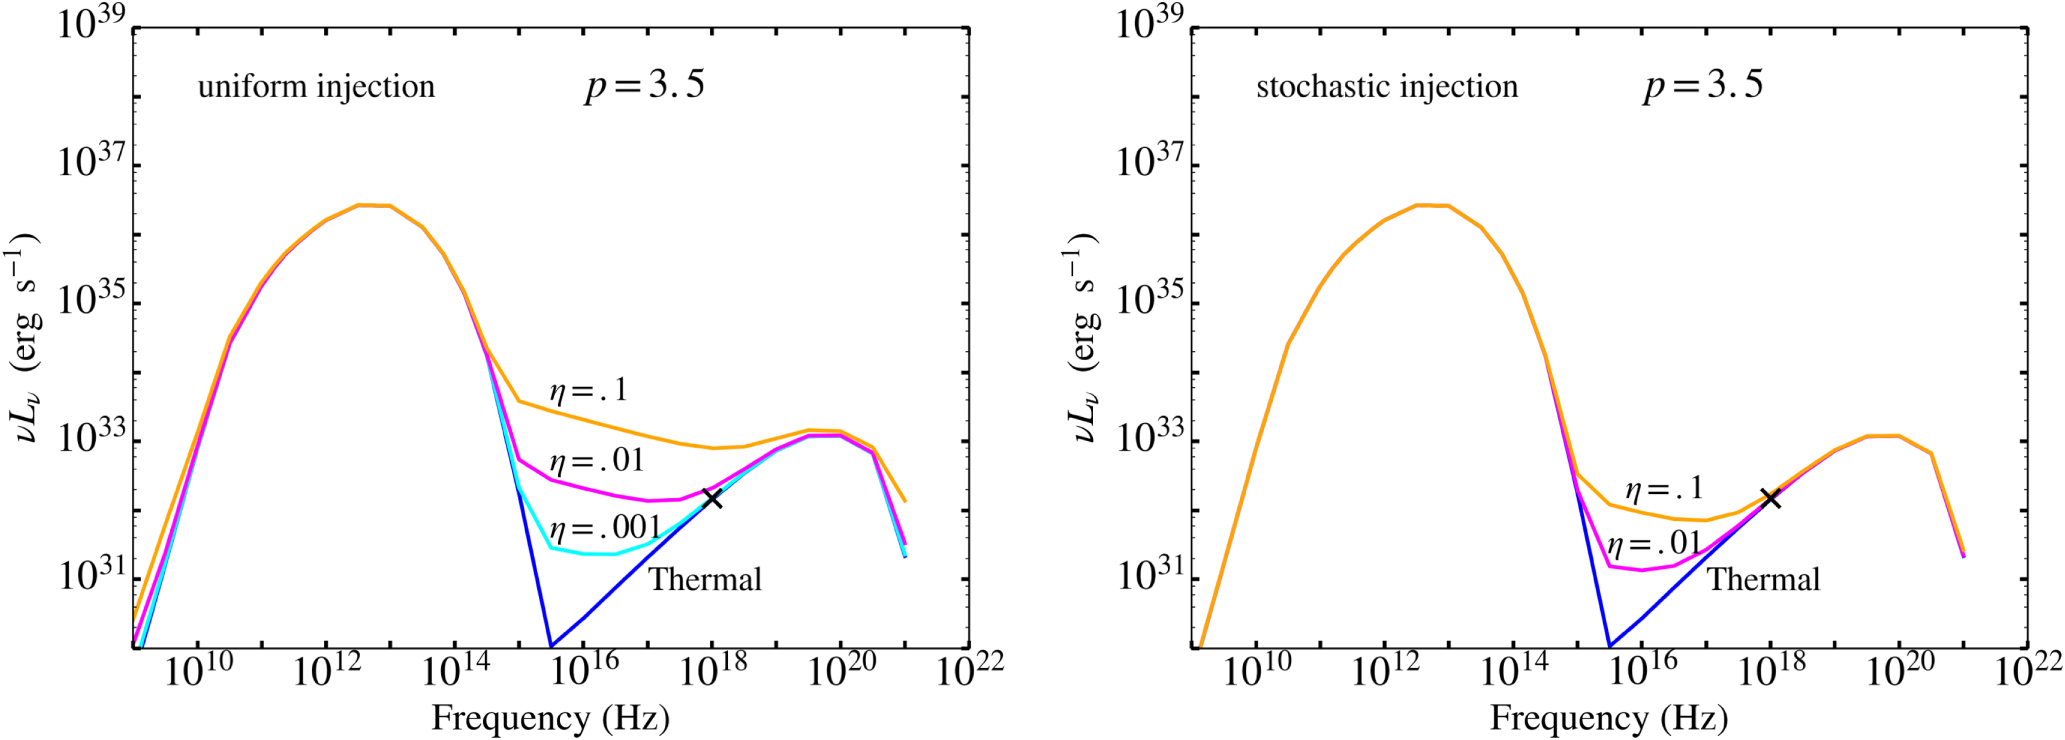
\includegraphics[angle=0,width=\columnwidth]{paper1_fig1}
\caption{Left: Spectra computed for quiescent (i.e., non-flaring) times for various values of the energy fraction of non-thermal electrons, $\eta$ with fixed power-law index, $p=3.5$, as well as for the purely thermal model.  In this configuration where the non-thermals only follow the thermal energy, the observed quiescent X-ray flux at $10^{18}$ Hz (depicted with an X) is exceeded even for moderate values of $\eta$.  Right: In this configuration, non-thermal electrons are injected in regions below $\beta=0.2$.  Localizing the non-thermal electrons to highly magnetized regions, where they are more likely to be accelerated, allows for significantly higher values of $eta$ while still accommodating the observed quiescent X-ray flux at $10^{18}$ Hz}
\label{fig1}
\end{figure}

In the right panel of Figure 1, we show the spectrum from the nonuniform stochastic model, where nonthermal electrons are localized to low-$\beta$ regions, again
with a power-law index of 3.5. Because of this localization, it is possible to accommodate higher fractions
of non-thermal electrons while still matching the quiescent thermal spectrum. In this model, it is possible
to inject almost 10\% of the total thermal energy into a
non-thermal electron distribution within the magnetized regions.
\section{X-Ray Variability: Stochastic Injection}


\begin{figure}
	\centering
	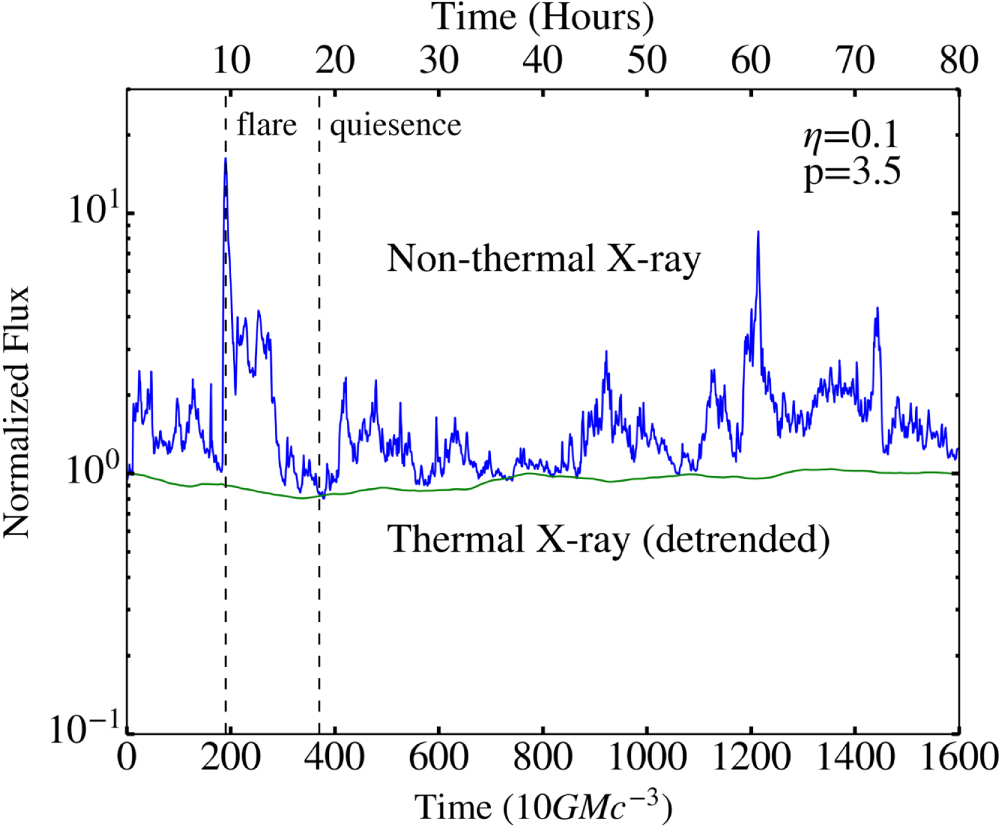
\includegraphics[angle=0,width=\columnwidth]{paper1_fig2}
	\caption{Thermal and non-thermal X-ray lightcurves.  The injection of non-thermal electrons into highly magnetized regions naturally produces significant variability due to the dynamic nature of magnetic fields in the accretion flow.}
	\label{fig2}
\end{figure}


\begin{figure}
	\centering
	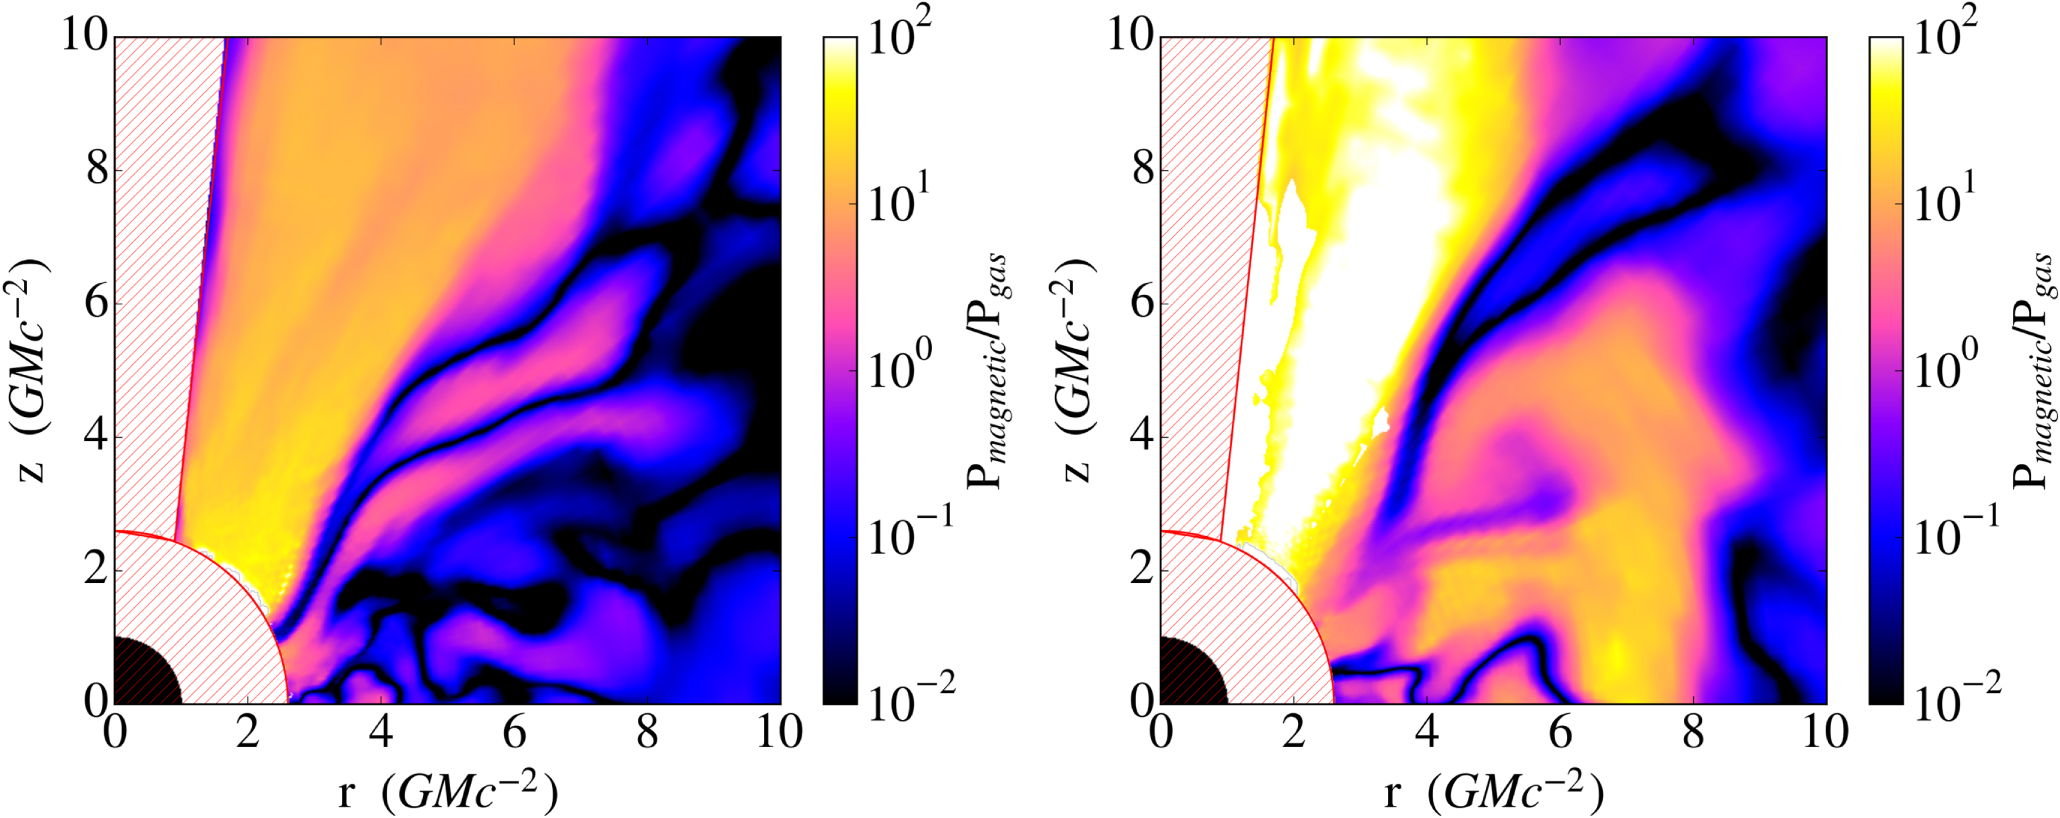
\includegraphics[angle=0,width=\columnwidth]{paper1_fig4}
	\caption{Left: Map of the ratio of the magnetic to gas pressure during a quiescent state in the simulation.  Cells near the pole and within the ISCO at $\sim 2.4 GMc^{-2}$ are excised due to numerical artifacts often occurring within these regions.  The black quarter-circle at the origin is the event horizon of the black hole.  Right: A large flux tube is present in the accretion flow during this flare, with high magnetization, resulting in a high ratio of pressures throughout a large portion of the disk. }
	\label{fig3}
\end{figure}

\begin{figure}
	\centering
	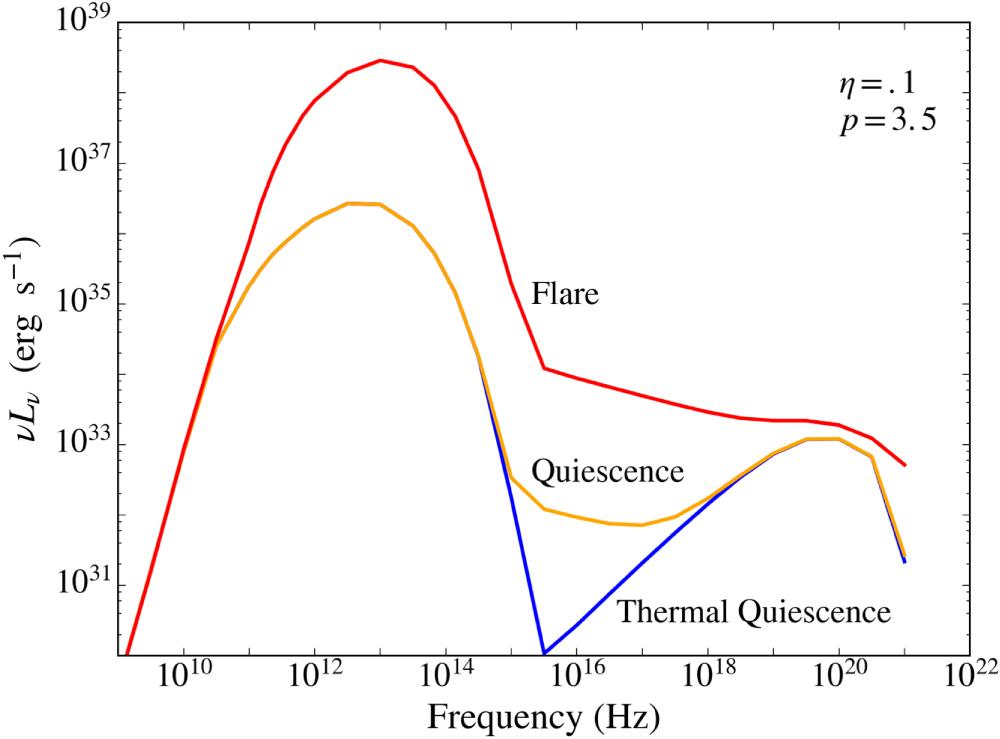
\includegraphics[angle=0,width=\columnwidth]{paper1_fig3}
	\caption{Spectra of the flaring and quiescent states depicted in Figure 3 in red and orange, respectively.  The purely thermal quiescent spectrum is shown for reference in blue. }
	\label{fig4}
\end{figure}

\begin{figure}
	\centering
	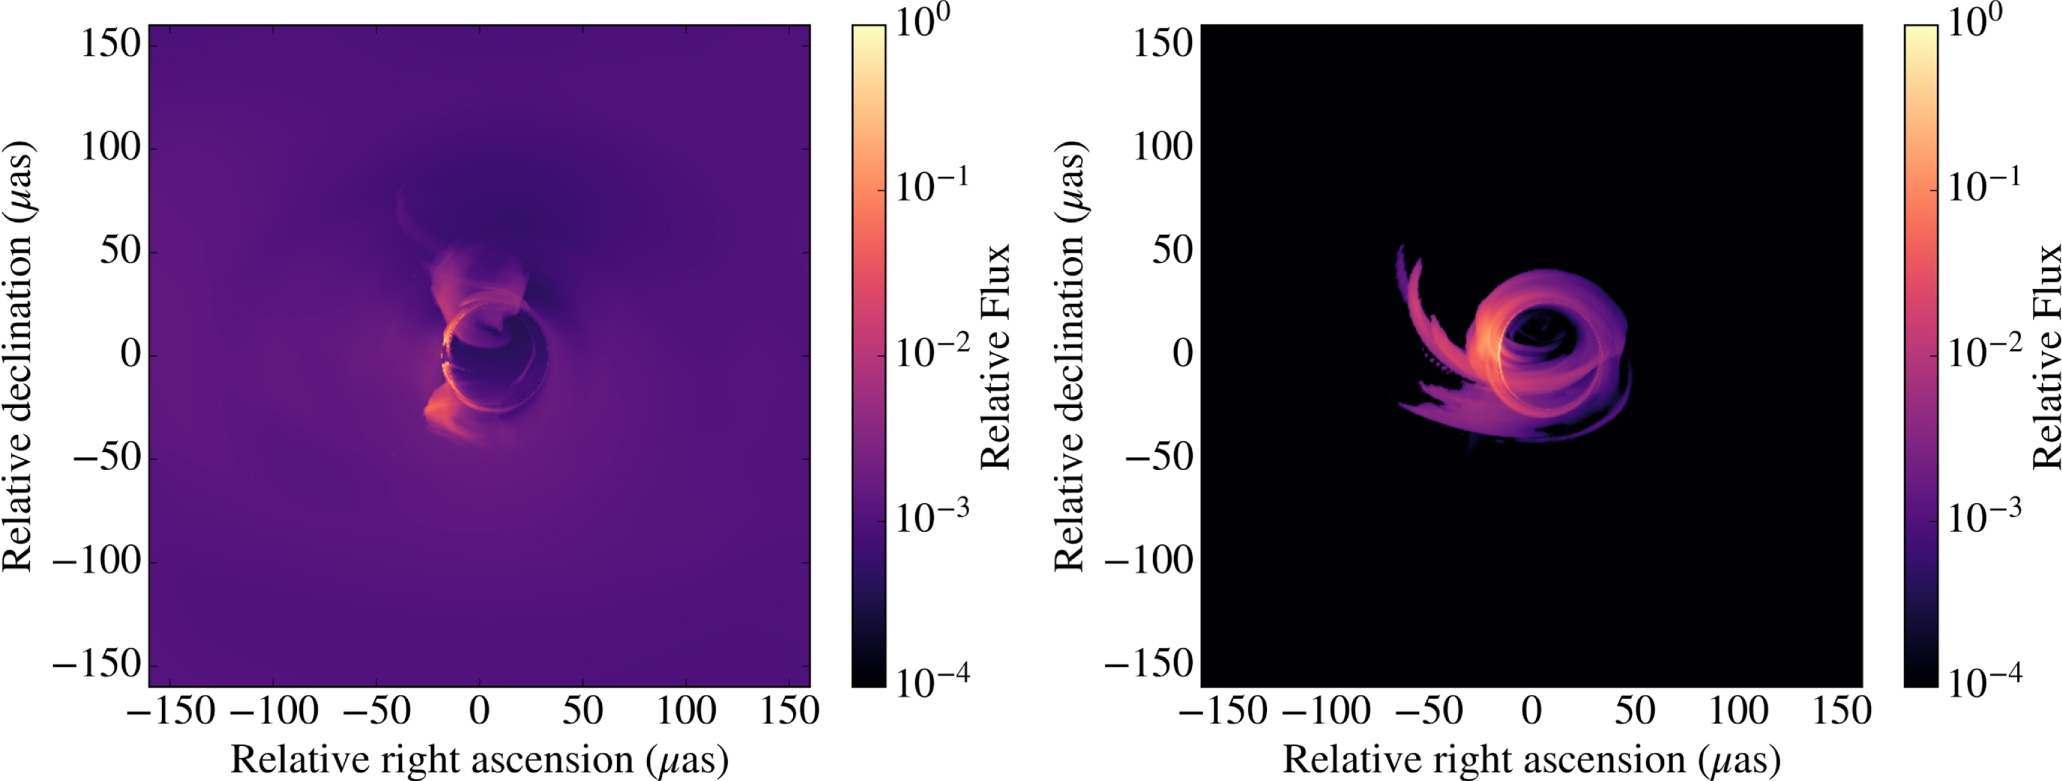
\includegraphics[angle=0,width=\columnwidth]{paper1_fig5}
	\caption{Left: Simulated image of quiescent X-ray (4.1 keV) emission. Fluxes are normalized to the maximum pixel value. Some
		structure is visible in the innermost regions of the image, where strong magnetic fields in the funnel close to the event horizon have
		associated non-thermal particles, and hence strong X-ray emission. We see that the extended Brehmsstrahlung emission comprises a
		significant fraction of the total flux during quiescence. Right: During the flare, emission is heavily dominated by the innermost part of the
		accretion flow; the relative contribution from the halo of Bremsstrahlung emission is negligible during flares.}
	\label{fig5}
\end{figure}

Apart from providing a more natural match to quiescent-state constraints, another interesting result
of using the $\beta$-dependent description of non-thermal electron injection is that it produces significant X-ray
variability. Perhaps this is not surprising, since the non-thermal electrons will trace magnetic flux tubes,
which are dynamic structures, constantly being formed, sheared, and moving throughout the flow. If one of these
flux tubes crosses a caustic behind the black hole, it will result in an additional amplification of the flux, and
since these tubes are emitting primarily non-thermal synchrotron radiation in the X-rays, they will cause X-ray
flares. We explore this variability in Figure \ref{fig2}, where we show the effect of stochastic injection of non-thermal electrons and compare it to a purely thermal model. In the nonthermal lightcurve, we see both persistent variability as
well as 4 large flares during the $\sim$80 hours of simulation. In the largest flares, the flux increases by a factor of $\sim 10$
compared to quiescence. The magnetically dominated regions responsible for these flares live for about 5000
seconds, which sets the timescale of the flares in this figure. There is indeed a stark contrast between this
result, which takes into account acceleration in low-$\beta$ regions, and the purely thermal model, which shows no variability.  We now investigate the properties of the magnetic structures in the innermost regions of the accretion flow
to further pinpoint the localization and time evolution of the flares. Figure \ref{fig3} shows the ratio of the magnetic
to the gas pressure throughout the inner flow during a
quiescent state and during the strongest flare from the
simulation. We see that this flare is caused by a large
magnetic flux region developing in the flow with $\beta < \beta_t$.
Due to the large spatial extent of this tube, many nonthermal electrons are injected, causing a sudden increase
in the X-ray flux. In contrast, during quiescence, the only
region with a significant number of non-thermal electrons
is in the funnel, which typically has a fairly uniform and
strong magnetic field. This only contributes a small flux
and results in low level variability.
Figure \ref{fig4} depicts the spectra of the flaring and quiescent
states from the simulation. During quiescence, the nonthermal emission is not especially prominent; its nature is
largely obscured by the thermal emission dominating at
most wavelengths. During the flare, however, the powerlaw nature of the non-thermal emission becomes more
evident.
In Figure 5, we show the X-ray images of our model
during flaring and quiescent states. The images show
the relative contribution to the overall flux from various
parts of the accretion flow. During quiescence, we find
that while there is some contribution to the X-ray flux

from a small population of non-thermal particles in the
funnel, the extended Bremsstrahlung emission accounts
for the majority of the total (i.e., integrated over the entire image) observed flux. During a flare, the emission is
heavily dominated by non-thermal electrons in the inner
accretion flow, rendering the Bremsstrahlung flux negligible. The difference in the localization of the X-rays
between the non-thermal and thermal models is responsible for their different variability properties.

\section{Comparison to Observations}
By interpreting observations of Sgr A* in the context of our GRMHD simulations, we begin to place constraints on the population of non-thermal electrons in the radiatively inefficient accretion flow and gain insight into their injection mechanisms. We employed two configurations for non-thermal electron injection, one in which the non-thermal electrons simply track the thermal energy everywhere throughout the flow and another where the non-thermal electrons are injected solely into regions of high magnetization. From the first model we are able to place tight constraints on the fraction of steady-state non-thermal electrons that may exist throughout the flow by comparing the simulations to the observed quiescent X-ray flux. The second model localizes non-thermal electrons to a much smaller region, allowing their local energy density to be much higher than the uniform model (by about 2 orders of magnitude) while still matching the
observed quiescent X-ray flux.


\begin{figure}
	\centering
	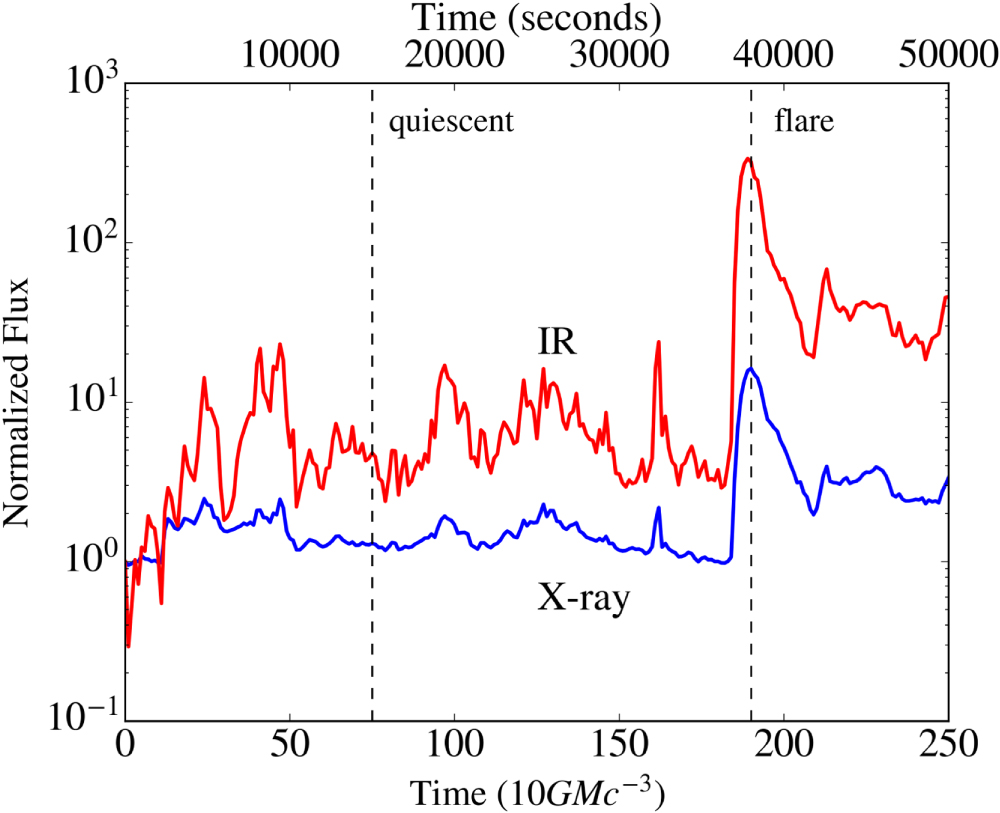
\includegraphics[angle=0,width=\columnwidth]{paper1_fig6}
	\caption{IR and X-ray lightcurves zoomed in on the first 250 timesteps of the simulation.  Each curve is normalized to a fiducial quiescent flux.  Note the strong and rapid variation in the IR flux and moderate variability in the X-ray.  The IR flaring has been described in \citet{chan2015b}.  The includsion of non-thermal electrons in highly magnetized regions has produced significant X-ray variability which was previously unseen.}
	\label{fig6}
\end{figure}

\begin{figure}
	\centering
	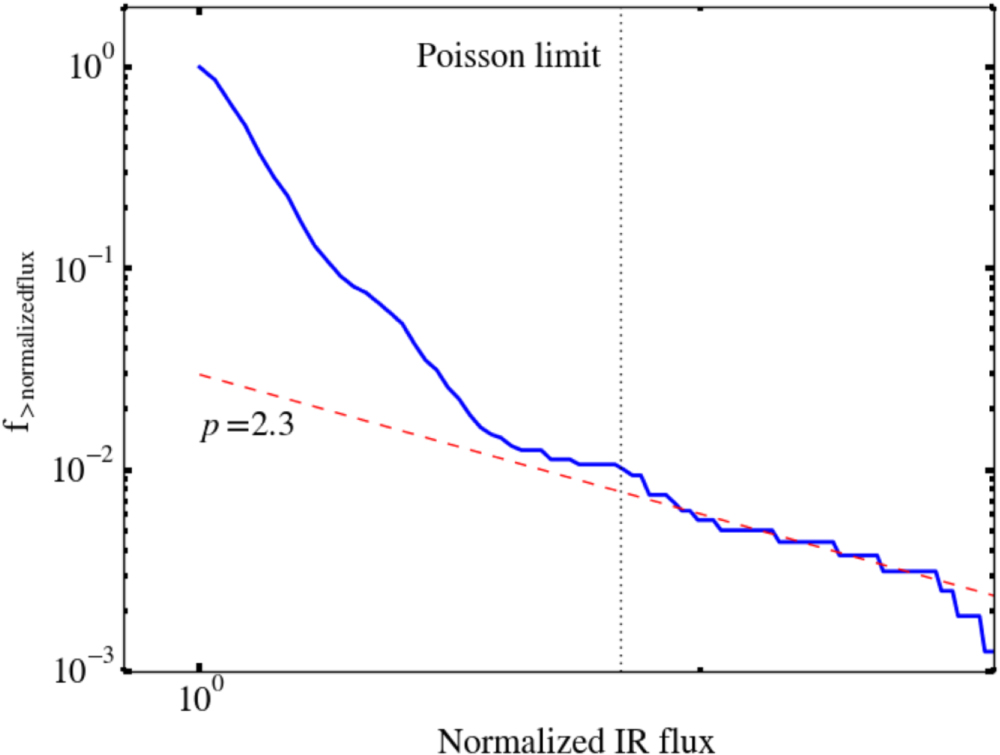
\includegraphics[angle=0,width=\columnwidth]{paper1_fig7}
	\caption{X-ray flux distribution, accounting for a constant quiescent background.  At high fluxes, the flare distribution resemble a power-law with an index of $\sim 2.3$.  Using the Poisson rate and binning reported in \citet{neilsen2015} for the Chandra observations used in that study, we estimate what would be the upper end of the Poisson-dominated regime, depicted with a vertical dotted line.}
	\label{fig7}
\end{figure}

\begin{figure}
	\centering
	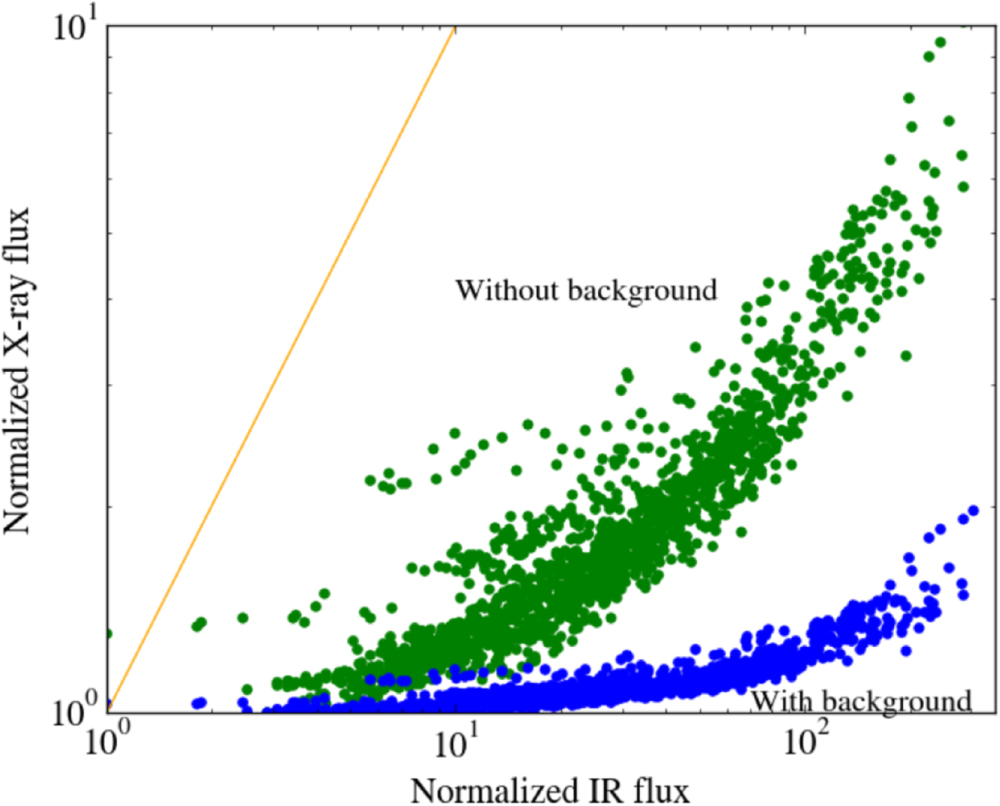
\includegraphics[angle=0,width=\columnwidth]{paper1_fig8}
	\caption{IR vs. X-ray flux, accounting for a constant quiescent background of X-ray flux (blue), and purely for the inner accretion flow (green).  The orange line depicts a correlation with a slope of unity.  The addition of the queiscent background decreases the X-ray variability by a factor of $\sim 10$.  We see a general trend of higher IR fluxes being associated with relatively high X-ray fluxes.}
	\label{fig8}
\end{figure}



We find that X-ray variability is a generic result of constraining the non-thermal electrons to highly magnetized regions. This is because the magnetic field is
dynamic throughout the flow, generating magnetic flux tubes, which are in a constant state of being formed, sheared, becoming buoyant, and leaving the disk. The
dynamic nature of these flux tubes combined with strong lensing effects from the black hole generate both persistent variability as well as flaring events.
X-ray flares in our simulations are always coincident with IR flares, but there are numerous IR flares without
X-ray counterparts, as shown in Figure \ref{fig6}, which qualitatively matches observations. In this figure, we have zoomed in to the first 250 timesteps of the simulation in order to more clearly illustrate the relationship between the IR and X-ray lightcurves. During this time span,
we observe about 5 IR flares over the stochastically variable background and one significant X-ray flare. From our simulation we find that there are about 5 IR flares per X-ray flare and a rate of one X-ray flare per 72,000 seconds, over the entire simulation. Over the course of
3 million seconds of observation with Chandra, 39 Xray flares were observed, corresponding to one flare every $\sim$77,000 seconds. Observations Sgr A* show that,
for every X-ray flare, there are about 4 NIR flares (e.g., \citealt{genzel2003, eckart2006}). These numbers
are in rough agreement with our results. In order to compare flare statistics from our simulations to observations more directly (e.g., through flux
distributions reported in Neilsen et al. 2015), we need to account for the fact that only  $\sim 10\%$ of the X-ray
emission from Sgr A* comes from the inner accretion flow (Neilsen et al. 2013). In Figure \ref{fig7}, after adding a
constant background equal to 90\% of the observed quiescent flux to our lightcurve from Figure 2, we plot the
flux distribution in our simulations. We find that the flare distribution resembles a power-law with an index of
around 2.3, while the lower-level variability does not have an obvious structure. Neilsen et al. (2015) reports only
Poisson variability at low fluxes, and power-law behavior at high fluxes, with a power-law index of 1.92. This is
roughly consistent with our simulated flux distribution. Our simulations, however, do not account for the Poisson photon counting noise, and also do not show as large of a range of variability. The latter is likely due to the
relatively short duration of our simulation that did not capture many rare, high flux events.
We estimate the level of the Poisson noise, below which we expect our simulated flux distribution to deviate significantly from observations. We take the reported photon counting rate ($Q = 5.24$ cts/ks) and binning ($b = 300$ s) from Neilsen et al. (2015) and calculate the typical fractional Poisson error, $\epsilon=1/\sqrt{Qb}=0.79$. Normalizing our lowest level of emission to 1, we see that counting noise
will dominate the observed variability from 1 to $1+\epsilon$,
setting the lower limit from which we expect our simulations to reproduce the flux distribution.
We further explore the relationship between IR and Xray fluxes in Figure \ref{fig8}. The largest IR flares correspond
to the largest X-ray flares, but there is much more variability in the IR than the X-rays. In our simulations,
anytime a flux tube appears and crosses a caustic there
will be an IR flare due to the synchrotron emission from
the thermal electrons. However, only the most highly
magnetized flux tubes will have non-thermal electrons
associated with them and will generate an X-ray flare.
The effect of the $\beta$ threshold is to pick out a subset of all
the magnetic flux tubes, ones with conditions suitable for
reconnection to occur. The particular threshold we use is
motivated by \citet{liguo2015}, who showed a non-thermal
component being generated for $\beta < 0.2$. As a result, IR
variability is much more significant, since there is thermal synchrotron associated with all flux tubes, whereas
particle acceleration and hence X-ray emission only occurs for a particular subset of the tubes. Additionally,
we see that the flux tubes responsible for the largest IR
flares are the same structures responsible for the largest
X-ray flares. This is unsurprising given the strong scaling
of synchrotron emissivity with magnetic field; the most
highly magnetized flux tubes radiate copiously in the IR
due to the high magnetic fields, and also act as sites of
efficient reconnection, generating strong X-ray flares.
\section{Conclusions}
In this paper, we explored the effects of incorporating non-thermal electrons into GRMHD simulations of
radiatively inefficient accretion flows. We found that
X-ray variability is a generic result of constraining the
non-thermal electrons to highly magnetized regions and
that the timescales associated with electron cooling are
comparable to the observed flare duration. This analysis is model-dependent, since the synchrotron radiation
from non-thermal electrons depends on the strength and
topology of the magnetic field, which will impact the constraints we place on the quiescent energy budget of the
non-thermal electrons. Our analysis of cooling timescales
are also likely to differ across models. For model B with
only inflowing velocities within 10 gravitational radii, we
found that flares are unlikely to originate from the funnel since the inward radial velocities were too large to
explain the X-ray flares lasting many thousands of seconds. We will explore the role of non-thermal electrons
in producing the variability for different magnetic field
configurations and black hole spins in a future study.
In the context of model B, which has matched many
observational constraints, from the quiescent broadband
spectrum to the variability properties, we find that Xray flares likely originate from magnetic flux tubes in the
disk, where centrifugal support allows the non-thermal
electrons to remain in the flow for many thousands of seconds while radiating away their energy via synchrotron
emission. The flare lengths are hence set by the synchrotron cooling timescales. The properties of the Xray variability from this model are consistent with observations: X-ray flares are always coincident with IR
flares, there are many more IR flares without associated
X-ray counterparts, and the timescales associated with
the flares are comparable to the observed flare duration.
\chapter[Quantifying Reconnection Current Sheets in GRMHD Simulations of Sgr~A*]
{chapter3}
\chapter[Electron and Proton Acceleration in Trans-relativistic Magnetic Reconnection: Dependence on Plasma Beta and Magnetization]
{chapter4}
\chapter[The Mechanism of Electron Injection and Acceleration in Trans-relativistic Reconnection]
{chapter5}



% Include the various appendices
\appendix
\chapter{Extra Stuff}

%\begin{figure}
%\centering
%\includegraphics[angle=0,width=\columnwidth]{fig1.pdf}
%\caption[]{}
%\label{fig1}
%\end{figure}


% Switch the spacing to single-spaced for the references
\renewcommand{\baselinestretch}{1}		% chaning the value
\small\normalsize						% switch size to make the value take

% Create the References list
\bibliographystyle{uabibnat}
\bibliography{bibliography}

\end{document}
